\documentclass{simplesnt}

\usepackage{kotex}
\usepackage[korean]{datetime2}
\usepackage{xcolor}
\usepackage{caption}
\usepackage{tcolorbox}
\usepackage{tikz}

\DTMsetdatestyle{iso} 


%% Helpful packages

\usepackage{listings}
\lstset{basicstyle = \small\ttfamily, breaklines}

\usepackage{tabularray}
\UseTblrLibrary{booktabs}

\usepackage{metalogo} % For XeTeX logo
\usepackage{kotex-logo}

\newcommand*{\presentfont}[1]{{\fontspec{#1}#1}}
\ExplSyntaxOn
\bool_if:nF { \sys_if_engine_xetex_p: || \sys_if_engine_luatex_p: }
  { \newcommand*{\fontspec}[1]{} }
\ExplSyntaxOff

\title{\texttt{분석기 취약점 파고들기}}
\author{정원준}

\begin{document}

\setcounter{framenumber}{5}

\section{걱정거리}

\begin{frame}[c, fragile]
  \frametitle{너무 안전한 분석기}
  
\includegraphics[width=\linewidth]{img/지구.png}
\end{frame}

\begin{frame}[c, fragile]
  \frametitle{엉성한 그물망}

  \setlength{\columnsep}{10pt}

  \begin{columns}[c]
    \column{0.5\textwidth}
    \vspace*{\fill}

    \lstset{
      language=Python,
      escapeinside={(*@}{@*)}, % ← 이 줄 추가!
      basicstyle=\ttfamily\small,
      lineskip=2pt,
      columns=fullflexible,
    }

    \hspace*{\fill} % 왼쪽 여백 채우기
    \centering % ← 추가
    \hfill
    \begin{minipage}{0.9\linewidth} % 코드가 너무 길면 1.0 대신 0.9 정도
    \begin{lstlisting}
x = int(input())

if x < 0:
    x = -x

print(x) // x >= 0
    \end{lstlisting}
    \end{minipage}
    \hspace*{\fill} % 오른쪽 여백 채우기

    \vspace*{\fill}

    \column{0.5\textwidth}
    \vspace*{\fill}
    \vspace*{\fill}
  \end{columns}

\end{frame}


\begin{frame}[c, fragile]
  \frametitle{엉성한 그물망}

  \setlength{\columnsep}{10pt}

  \begin{columns}[c]
    \column{0.5\textwidth}
    \vspace*{\fill}

    \lstset{
      language=Python,
      escapeinside={(*@}{@*)}, % ← 이 줄 추가!
      basicstyle=\ttfamily\small,
      lineskip=2pt,
      columns=fullflexible,
    }
    \centering % ← 추가
    \hfill
    \begin{minipage}{0.9\linewidth} % 코드가 너무 길면 1.0 대신 0.9 정도
    \begin{lstlisting}
x = int(input())

if x < 0:
    x = -x

print(x) // x >= 0
    \end{lstlisting}
    \end{minipage}

    \vspace*{\fill}

    \column{0.5\textwidth}
    \vspace*{\fill}
    \lstset{
      language=Python,
      escapeinside={(*@}{@*)}, % ← 이 줄 추가!
      basicstyle=\ttfamily\small,
      lineskip=2pt,
      columns=fullflexible,
    }

    \hspace*{\fill}
    \centering % ← 추가
    \hfill
    \begin{minipage}{0.9\linewidth} % 코드가 너무 길면 1.0 대신 0.9 정도
    \begin{lstlisting}
x = int(input())

(*@\textcolor{red}{a = -x}@*)
if (*@\textcolor{red}{a < 0}@*):
    x = -x

print(x) // x >= 0 (*@\textcolor{red}{??}@*)
    \end{lstlisting}
    \end{minipage}
    \vspace*{\fill}
  \end{columns}

\end{frame}




\section{공격의 기대효과}

\begin{frame}[c, fragile]
  \frametitle{적대적 공격(Adversarial attack)}
  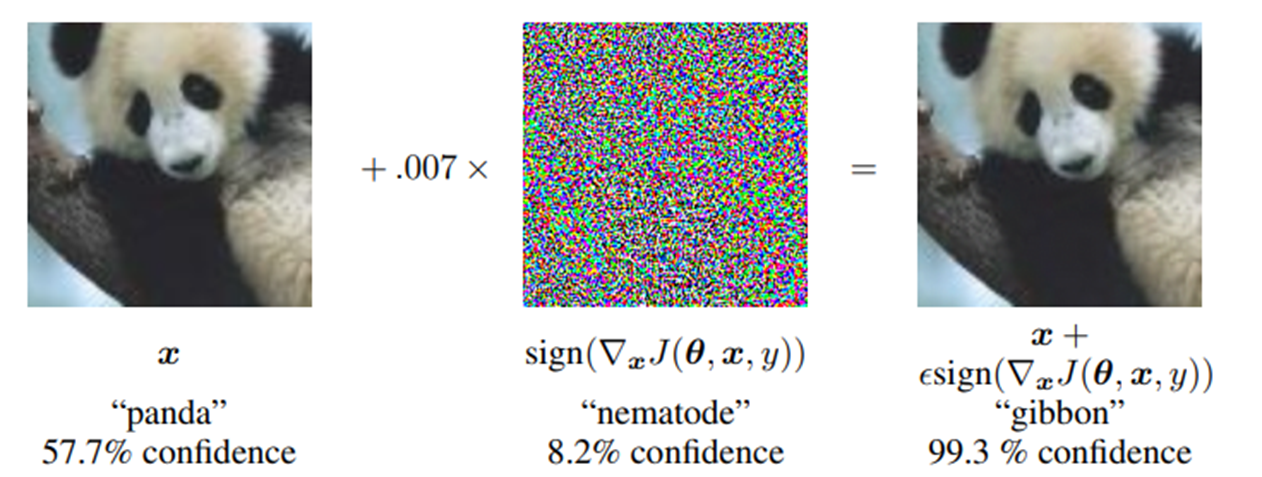
\includegraphics[width=\linewidth]{img/적대적공격.png}
  
  \vfill
  {\tiny\hfill Goodfellow, Ian J., Jonathon Shlens, and Christian Szegedy. ``Explaining and Harnessing Adversarial Examples.'' arXiv, 20 Mar. 2015, \href{https://arxiv.org/abs/1412.6572}{arxiv.org/abs/1412.6572} \hspace{0.5cm}}
\end{frame}

\begin{frame}[c]
  \frametitle{취약점 개선}

  % 첫 문장 상자 (가운데 정렬 + 문장 크기에 딱 맞게)
  \begin{center}
    \begin{tcolorbox}[
      colback=gray!10,
      colframe=black,
      box align=center,
      halign=center,
      sharp corners
    ]
    분석기의 치명적인 약점 파악
    \end{tcolorbox}
  \end{center}

  % 굵은 화살표
  \vspace{0.5em}
  \begin{center}
    \tikz{\draw[->, ultra thick] (0,0) -- (0,-0.8);}
  \end{center}
  \vspace{0.5em}

  % 두 번째 문장 상자
  \begin{center}
    \begin{tcolorbox}[
      colback=gray!10,
      colframe=black,
      box align=center,
      halign=center,
      sharp corners
    ]
    약점 보완 방법 탐색
    \end{tcolorbox}
  \end{center}
\end{frame}

\section{마저 할 일}


\begin{frame}[c]
  \frametitle{마저 할 일}
  \begin{itemize}
      \item 프로그램 분석 숙제 마무리하기
      \vspace{1.5em}
      \item 여러 요약 방법에 따른 취약점 각각 찾아보기
      \vspace{1.5em}
      \item 일반화하기
  \end{itemize}
\end{frame}

\begin{frame}[c]
  \frametitle{일반화}

  튜링 완전한 언어 $L$, 실행 함수의 요약 규칙 $\#$, 축지법(widening operator) $\nabla$가 주어졌을 때,

  L에 해당하는 실행함수 $F$를 찾아

  귀납적으로 정의된 수열
\[
    X_0^{\#} = \perp^{\#}
\]
\[
    X_{i+1}^{\#} = X_i^{\#} \nabla F^{\#}(X_i^{\#})
\]
  이 
\[
    \lim_{i} X_i^{\#} = \top^{\#}
\]
  가 되게 하기.
  

\end{frame}


\definecolor{mydarkblue}{RGB}{32,56,61}

\setbeamercolor{background canvas}{bg=mydarkblue}
\setbeamercolor{normal text}{fg=white}
\setbeamercolor{frametitle}{fg=white}
\addtocounter{framenumber}{-1} % 마지막 슬라이드 번호를 하나 줄임
\appendix
\begin{frame}[c] % [c]는 내용 수직 가운데 정렬
  \centering
  {\Large \textcolor{white}{감사합니다}}
\end{frame}

\end{document}
